\documentclass[a4paper]{article}
\usepackage[utf8]{vietnam}
\usepackage{a4wide,amssymb,epsfig,latexsym,multicol,array,hhline,fancyhdr}
\usepackage{amsmath}
\usepackage{lastpage}
\usepackage[lined,boxed,commentsnumbered]{algorithm2e}
\usepackage{enumerate}
\usepackage{listings}
\usepackage{color}
\usepackage{graphicx}
\usepackage{array}
\usepackage{tabularx, caption}
\usepackage{multirow}
\usepackage{multicol}
\usepackage{rotating}
\usepackage{graphics}
\usepackage{geometry}
\usepackage{setspace}
\usepackage{epsfig}
\usepackage{tikz}
\usepackage{blindtext}
\usepackage{subcaption}
\usepackage{caption}
\usepackage{array}
\usetikzlibrary{arrows,snakes,backgrounds}
\usepackage{hyperref}
\usepackage{float}
\usepackage{makecell}
\usepackage{longtable}
\usepackage{xtab}
\usepackage{indentfirst}
\usepackage{zlmtt}
\usepackage{fancyvrb}
\usepackage{scrextend}
\usepackage{array}
\usepackage{caption}



\definecolor{red}{rgb}{0.6,0,0} 
\definecolor{blue}{rgb}{0,0,0.6}
\definecolor{green}{rgb}{0,0.8,0}
\definecolor{cyan}{rgb}{0.0,0.6,0.6}
\definecolor{white}{rgb}{255.0,255.0,255.0}
\definecolor{gamedev}{rgb}{0.145,0.55,0.8}



\DeclareCaptionFont{white}{\color{white}}
\DeclareCaptionFormat{listing}{\colorbox{gamedev}{\parbox{\textwidth}{\hspace{15pt}#1#2#3}}}
\captionsetup[lstlisting]{format=listing,labelfont=white,textfont=white, singlelinecheck=false, margin=0pt, font={bf,footnotesize}}

\newtheorem{theorem}{{\bf Theorem}}
\newtheorem{property}{{\bf Property}}
\newtheorem{proposition}{{\bf Proposition}}
\newtheorem{corollary}[proposition]{{\bf Corollary}}
\newtheorem{lemma}[proposition]{{\bf Lemma}}





\hypersetup{urlcolor=blue,linkcolor=black,citecolor=black,colorlinks=true} 




% Header and Footer
\setlength{\headheight}{40pt}

\pagestyle{fancy}

\fancyhead{} % clear all header fields
\fancyhead[L]{
 \begin{tabular}{rl}
    \begin{picture}(25,15)(0,0)
    \put(0,-5){
\includegraphics[width=10mm, height=10mm]{Images/bku_logo.jpg}}

   \end{picture}

% 	\begin{tabular}{l}
% 		\textbf{\bf \ttfamily Ho Chi Minh City University of Technology}\\
% 		\textbf{\bf \ttfamily Faculty of Computer Science and Engineering}\\
% 	\end{tabular} 	
\vspace{0.25cm}
 \end{tabular}
}

% \fancyhead[R]{
% 	\begin{tabular}{l}
% 		\tiny \bf \\
% 		\tiny \bf 
% 	\end{tabular}  }

\fancyfoot{} % clear all footer fields
% \fancyfoot[R]{\scriptsize \ttfamily Page {\thepage}/\pageref{LastPage}}
\fancyfoot[R]{\thepage}

\renewcommand{\headrulewidth}{0.3pt}
\renewcommand{\footrulewidth}{0.3pt}

% Mục lục
\setcounter{secnumdepth}{4}
\setcounter{tocdepth}{3}

\makeatletter
\newcounter {subsubsubsection}[subsubsection]
\renewcommand\thesubsubsubsection{\thesubsubsection .\@alph\c@subsubsubsection}
\newcommand\subsubsubsection{\@startsection{subsubsubsection}{4}{\z@}%
	{-3.25ex\@plus -1ex \@minus -.2ex}%
	{1.5ex \@plus .2ex}%
	{\normalfont\normalsize\bfseries}}
\newcommand*\l@subsubsubsection{\@dottedtocline{3}{10.0em}{4.1em}}
\newcommand*{\subsubsubsectionmark}[1]{}
\makeatother

\renewcommand*\contentsname{Mục lục}
\renewcommand*\refname{References}

\changefontsizes{13pt}


% Report
% Report
% Report
% Report
\begin{document}


    \begin{titlepage}

    \begin{center}
	ĐẠI HỌC QUỐC GIA THÀNH PHỐ HỒ CHÍ MINH \\
	TRƯỜNG ĐẠI HỌC BÁCH KHOA \\
	KHOA KHOA HỌC - KỸ THUẬT MÁY TÍNH
\end{center}
	

\begin{figure}[h!]
	\begin{center}
		
\includegraphics[width=4.5cm]{Images/bku_logo.jpg}
	\end{center}
\end{figure}
	    
\begin{center}
	\begin{tabular}{c}
		\multicolumn{1}{l}{\textbf{{\Large  ĐỀ CƯƠNG LUẬN VĂN TỐT NGHIỆP ĐẠI HỌC}}}            \\
		                                                                                                        \\
		\hline                                                                                                  
		                                                                                                        \\
		\multicolumn{1}{l}{\textbf{{\LARGE MẠNG XÃ HỘI}}} \\
		\multicolumn{1}{l}{\textbf{{\LARGE CỘNG ĐỒNG YÊU THÍCH CHỤP ẢNH}}} \\
		                                                                                                        \\
		\hline                                                                                                  
		\multicolumn{1}{l}{\textbf{\Large NGÀNH: KHOA HỌC MÁY TÍNH}}                                       
			                                                                                                        
	\end{tabular}
\end{center}
	    




% \begin{center}
% 	\begin{tabular}{c}
% 												\\
% 		\textbf{\Huge E-COMMERCE}               
% 												\\\\
% 		\hline                                  
% 												\\
% 		\textbf{{\Huge Concept Course Website}} \\
% 		\textbf{{\Huge Concept Course Website}} \\
% 												\\
% 		\hline                                  
% 	\end{tabular}
% \end{center}

    % \vspace{1.5cm}
	
\begin{table}[h]
    \begin{tabular}{rrl}
        \hspace{3cm} & \large{\textbf{\underline{Giáo viên hướng dẫn:}}} & \large{TS. Lê Thị Bảo Thu}       \\ \\
        & \large{\textbf{\underline{Sinh viên thực hiện:}}} 
        & \large{Trịnh Duy Hưng - 1913652} \\
                        &                                                          & \large{Đặng Quốc Thanh - 1915083} \\
                        &                                                          & \large{Hà Quốc Lương - 1914078}   \\ \\
    \end{tabular}
\end{table}
    
	\begin{center}
		Thành phố Hồ Chí Minh, tháng 12 năm 2022
	\end{center}
\end{titlepage}
    
    \newpage
        
    \centerline{{\bfseries \LARGE Lời cam đoan}}

\bigskip
\bigskip

    Chúng tôi xin cam đoan đây là công trình nghiên cứu của riêng chúng tôi
dưới sự hướng dẫn của TS. Lệ Thị Bảo Thu. Nội dung nghiên cứu và các kết
quả đều là trung thực và chưa từng được công bố trước đây. Các số liệu được sử
dụng cho quá trình phân tích, nhận xét được chính chúng tôi thu thập từ nhiều
nguồn khác nhau và sẽ được ghi rõ trong phần tài liệu tham khảo.\par
Ngoài ra, chúng tôi cũng có sử dụng một số nhận xét, đánh giá và số liệu
của các tác giả khác, cơ quan tổ chức khác. Tất cả đều có trích dẫn và chú thích
nguồn gốc.\par
Nếu phát hiện có bất kì sự gian lận nào, chúng tôi xin hoàn toàn chịu trách
nhiệm về nội dung thực tập tốt nghiệp của mình. Trường đại học Bách Khoa
thành phố Hồ Chí Minh không liên quan đến những vi phạm tác quyền, bản
quyền do chúng tôi gây ra trong quá trình thực hiện

    
    \newpage
        
    \centerline{{\bfseries \LARGE Lời ngỏ}}

\bigskip
\bigskip

Lời đầu tiên, chúng tôi xin được tỏ lòng biết ơn sâu sắc đối với sự hướng
dẫn, quan tâm của TS. Lê Thị Bảo Thu. Sự quan tâm và hướng dẫn của thầy
đã giúp chúng tôi có được sự tiếp cận với những kiến thức mới hơn và định
hướng tốt hơn cho quá trình nghiên cứu và thực hiện đề tài.\par
Xin chân thành cảm ơn các thầy, cô thuộc khoa Khoa học và Kỹ thuật Máy
Tính - trường Đại Học Bách Khoa - Đại Học Quốc Gia TP.HCM đã tận tình
giảng dạy cho chúng tôi trong thời gian học tập tại trường.\par
Cuối cùng, chúng tôi kính mong sự chỉ dẫn và đóng góp của các thầy, cô để
hoàn thiện hơn đề tài nghiên cứu này. Xin chân thành cảm ơn!
    
    \newpage

    \tableofcontents

    \newpage

    \section{Tổng quan}

\subsection{Lý do lựa chọn đề tài}
Mạng xã hội đã trờ thành một phần không thể thiếu trong cuộc sống của chúng ta ngày nay. 
Nó là một công cụ giao tiếp có giá trị với những người khác trong nước và trên toàn thế giới, cũng như để chia sẻ,
 tạo và truyền bá thông tin.\par 
Hiện nay, với sự phát triển mạnh mẽ của các thiết bị điện tử và ngành du lịch, khách tham quan từ nhiều nơi khác nhau 
sẽ đến những điểm du lịch để có những trải nghiệm mới, việc chụp ảnh để lưu giữ lại kỉ niệm cùng với người thân, bạn bè 
từ đó cũng là điều không thể thiếu. Vậy chúng ta lưu giữ và chia sẻ hình ảnh ở đâu?\par 
Instagram hiện nay được cho là nền tảng mạng xã hội phổ biến nhất để lưu giữ, xem những hình ảnh, video từ bạn bè và 
những nhân vật công chúng mà chúng ta thấy hấp dẫn và thú vị. Bên cạnh đó, Pinterest là website rất phổ biến để lưu giữ, 
chia sẻ ảnh theo dạng mạng xã hội, dùng để post và phân loại dưới dạng các đính kèm.
Cả hai mạng xã hội đều đang có một nhược điểm khác nhau. Instagram thì không tập trung toàn bộ vào chia sẻ hình ảnh, 
các chức năng mạng xã hội chỉ dừng ở việc chia sẻ, nhắn tin. Trong khi đó thì Pinterest tập trung vào mảng hình ảnh nhưng lại 
thiếu các chức năng của mạng xã hội.\par
Do đó, chúng tôi muốn xây dựng một mạng xã hội dành cho cộng đồng những người yêu thích chụp ảnh. Tại đây, mọi người 
có thể chia sẻ những bức ảnh đẹp do chính họ chụp được, những công thức riêng cho một bức ảnh đẹp, những kiến thức về máy ảnh 
và cách chụp ảnh. Ngoài ra, người dùng có thể tìm kiếm,  bình luận, chia sẻ, nhắn tin,  lập các hội nhóm chung sở thích để chi sẻ, 
học hỏi kinh nghiệm. Mạng xã hội này sẽ khắc phục nhửng nhược điểm của hai mạng xã hội trên, kết hợp những ưu điểm để tạo ra một nơi 
mà những người yêu thích chụp ảnh chắc chắn sẽ tìm tới.


\subsection{Lý do lựa chọn đề tài}
Từ những nội dung trên, một số vấn đề được đề cập và giải quyết trong đề tài này:
    \begin{itemize}
        \item Làm thế nào bảo vệ bản quyền cho ảnh của người dùng và cho nền tảng?
        \item Làm cách nào để xây dựng giải thuật tìm kiếm dựa vào ảnh tương tự?
        \item Làm sao để ứng dụng đáp ứng được mục tiêu: là nơi để cộng đồng đam mê nhiếp ảnh có thể chia sẻ ảnh và kinh nghiệm chụp ảnh?
        \item Những tính năng nào của mạng xã hội đòi hỏi có trong ứng dụng?
    \end{itemize}

Để thực hiện được mục tiêu này, chúng tôi đã đề ra những nhiệm vụ cần phải giải quyết như sau:
    \begin{itemize}
        \item Nghiên cứu và ứng dụng auto watermarking, hoặc hạn chế người dùng chụp màn hình.
        \item Xây dựng nền tảng cung cấp đầy đủ các tính năng mạng xã hội và ưu tiên phát huy tối đa tính năng lưu giữ và chia sẻ hình ảnh.
        \item Xây dựng hệ thống ổn định và đáng tin cậy
    \end{itemize}


\subsection{Lý do lựa chọn đề tài}
Phạm vi nghiên cứu của đề tài nhóm sẽ tìm hiểu về lĩnh vực mạng xã hội, các nội dung về lĩnh vực nhiếp ảnh.\par
Đối tượng nghiên cứu chủ yếu của đề tài sẽ dành cho tất cả mọi người có yêu thích về nhiếp ảnh và 
có cơ hội muốn tìm hiểu về nhiếp ảnh, Instagram và Pinterest
    

    \newpage

    \section{Các mạng xã hội hiện nay}

\subsection{Instagram}

Instagram là một mạng xã hội chuyên chia sẻ hình ảnh và video trên IOS, Android và Windows phone, bản thân nó được thiết kế dựa trên cơ sở sáng tạo ra những bức ảnh đẹp và thu hút. Đồng thời, nó cũng cung cấp rất nhiều các chế độ chỉnh sửa ảnh và video khác nhau theo sở thích của người dùng.\\ \par

Năm 2010, Instagram nhanh chóng trở thành một trong những mạng xã hội phát triển nhất. Đến năm 2012, Instagram được Facebook mua lại, cuộc sáp nhập này giúp cho Instagram đạt được con số tăng trưởng người dùng nhanh hơn cả Facebook, Twitter hay Pinterest. Chỉ sau 1 năm sát nhập với 
 Facebook, mạng xã hội Instagram đã đạt tới con số 150 triệu người dùng mỗi tháng.\\ \par
\par

Instagram cũng được đánh giá là sử dụng rất đơn giản. Những người lớn tuổi cũng có thể dễ dàng sử dụng nó, chỉ cần chạm vào biểu tượng máy ảnh sau đó chụp cho mình một vài tấm ảnh rồi tải lên là được. Còn đối với giới trẻ hiện nay thì Instagram đã không còn quá xa lạ, đây là ứng dụng phổ biến, kênh truyền thông hiệu quả, có khả nắng thúc đẩy tương tác rất tốt. Vì thế Instagram rất dễ dàng tiếp cận với người dùng trên toàn cầu. \\ \par

Bạn có thể thỏa thích chia sẻ hình ảnh một cách an toàn với Instagram. Bạn có thể lựa chọn nhiều hình thức để chia sẻ hình ảnh như: Chia sẻ cho bạn bè hay thiết lập quyền riêng tư chỉ riêng bạn thấy. Hoặc bạn có thể sử dụng chức năng Share Direct để share hình ảnh này với duy nhất một người. Chứng tỏ Instagram rất tôn trọng việc riêng tư của người dùng.\\ \par 

Phía trên là một vài thông tin cơ bản, bên cạnh đó thì Instagram còn cung cấp rất nhiều tính năng nổi bật, chúng ta cùng tìm hiểu cụ thể về mạng xã hội này.\\ \par

\newpage
\textbf{Những tính năng nổi bật của Instagram:}
\begin{itemize}
    \item \textbf{Xem và chia sẻ ảnh, video.} Một bức ảnh, video đơn giản có thể nói lên hết những suy nghĩ và cảm xúc của bạn. Bạn dễ dàng xem và chia sẻ những bức ảnh, video thay lời muốn nói trên ứng dụng Instagram. Đặc biệt, bạn có thể xem lại những bức ảnh bạn đã like dễ dàng từ vài tuần đến vài tháng trước. Ngoài ra, bạn có thiết lập quyền riêng tư khi chia sẻ ảnh và video trên ứng dụng, bạn dễ dàng quản lý ai được quyền xem và like những bức ảnh, video của bạn.\par
    \begin{figure}[h!]
        \centering
        
\includegraphics[width=6cm]{Images/chapter 2/instagram/post_app.jpg}
        \caption{Bài đăng trên ứng dụng di động}
        \label{fig:my_label}
    \end{figure}
  
    \begin{figure}[h!]
        \centering
        
\includegraphics[width=12cm]{Images/chapter 2/instagram/post_web.png}
        \caption{Bài đăng trên web}
        \label{fig:my_label}
    \end{figure}
\\
\newpage
    \item \textbf{Công cụ tạo ảnh, video sống động.} Bạn dễ dàng chỉnh sửa ảnh và video bằng Instagram để có những bức ảnh đẹp nhất trước khi đăng lên bảng tin của mình. Với những công cụ chỉnh sửa đơn giản như các bộ lọc, hiệu ứng, bóng mờ, làm rõ nét, chỉnh sửa màu sắc… để có bức ảnh đẹp nhất.\\
\newpage
    \begin{figure}[h!]
        \centering
        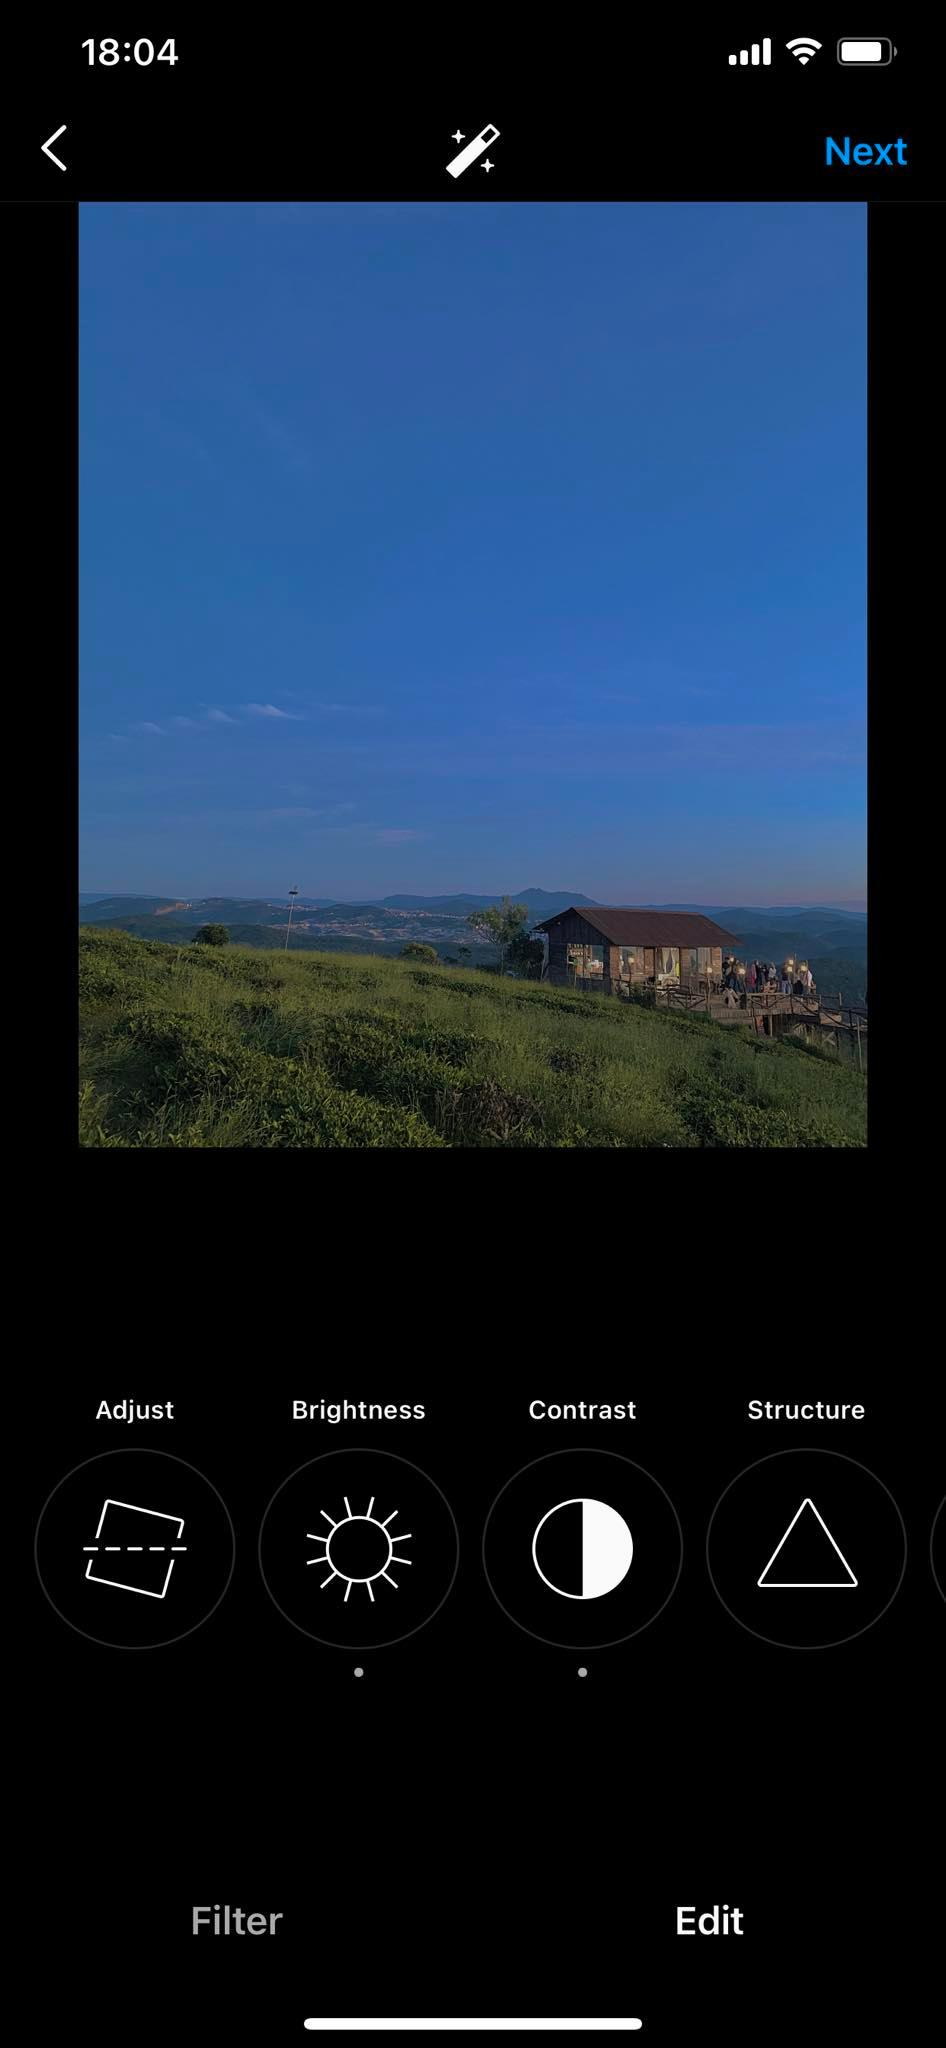
\includegraphics[width=7cm]{Images/chapter 2/instagram/edit_app.jpg}
        \caption{Chỉnh sửa ảnh trên ứng dụng di động}
        \label{fig:my_label}
    \end{figure}
    
    \begin{figure}[h!]
        \centering
        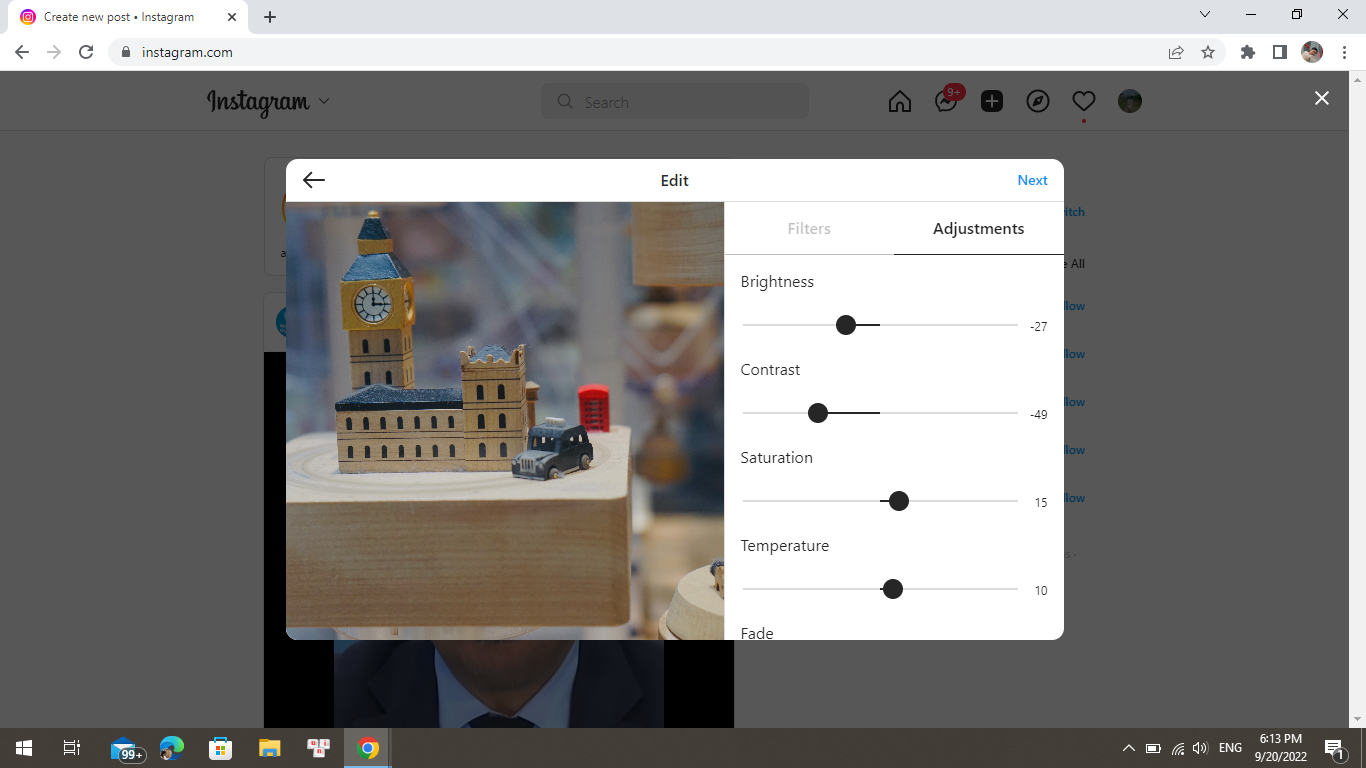
\includegraphics[width=13cm]{Images/chapter 2/instagram/edit_web.png}
        \caption{Chỉnh sửa ảnh trên web}
        \label{fig:my_label}
    \end{figure}
\\
\newpage
    \item \textbf{Tìm kiếm và khám phá nhiều nội dung từ cộng đồng, Reels.} Instagram là ứng dụng mạng xã hội phát triển rộng rãi trên toàn thế giới. Vì vậy, cũng như các ứng dụng mạng xã hội khác, bạn dễ dàng tìm kiếm và khám phá mọi thứ từ những bức ảnh, video trong được chia sẻ trên Instagram.\\
\newpage
    \begin{figure}[h!]
        \centering
        
\includegraphics[width=7cm]{Images/chapter 2/instagram/search_app.jpg}
        \caption{Tìm kiếm và khám phá nội dung trên ứng dụng di động}
        \label{fig:my_label}
    \end{figure}\
    
    \begin{figure}[h!]
        \centering
        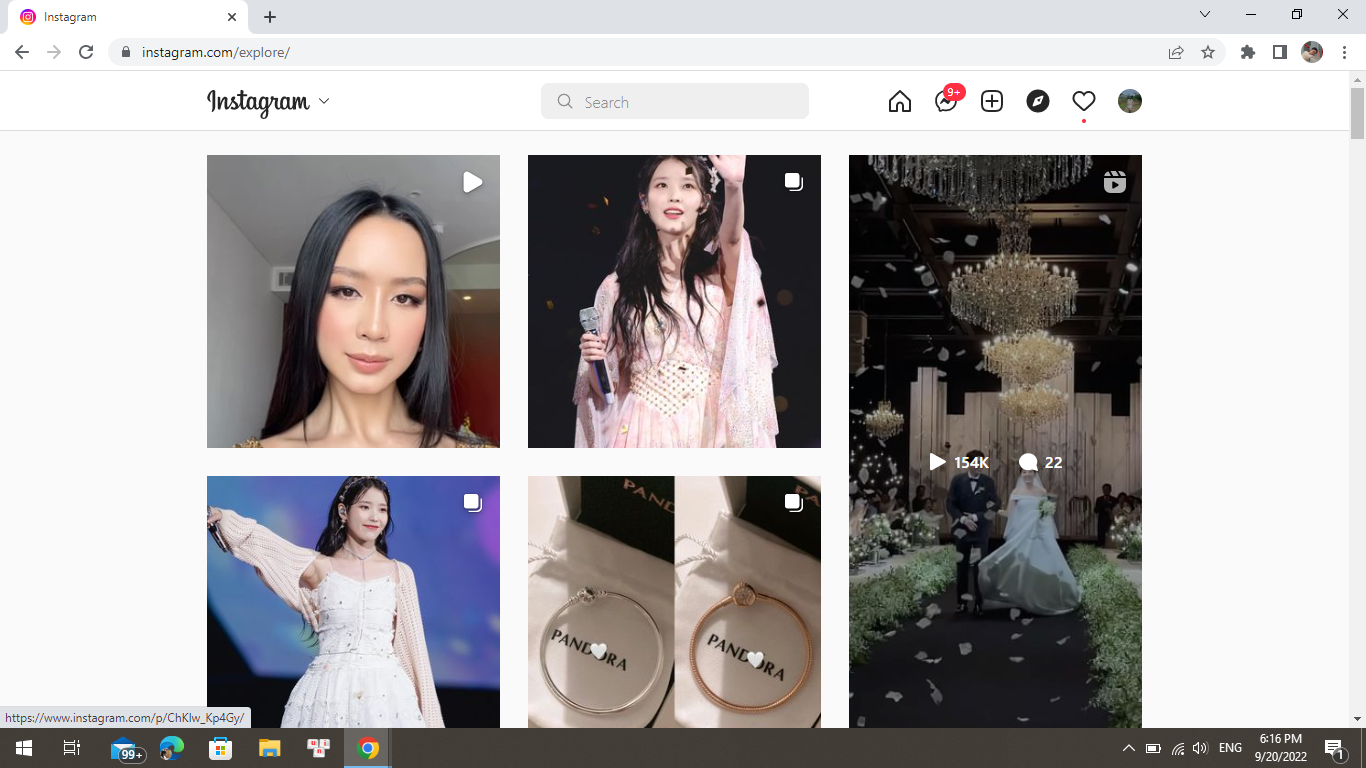
\includegraphics[width=13cm]{Images/chapter 2/instagram/search_web.png}
        \caption{Tìm kiếm và khám phá nội dung trên web}
        \label{fig:my_label}
    \end{figure}
\\
\newpage
    Ngoài ra reels của Instagram cũng được đánh giá là nơi chia sẻ video rất hot hiện nay.
    \begin{figure}[h!]
        \centering
        
\includegraphics[width=7cm]{Images/chapter 2/instagram/reel_app.jpg}
        \caption{Reels trên ứng dụng di động}
        \label{fig:my_label}
    \end{figure}
\\
\newpage
    \item \textbf{Đăng story và phát live stream dễ dàng.} Để chia sẻ những khoảnh khắc đáng nhớ, những hiệu ứng có sẵn của ứng dụng sẽ giúp bạn tạo ra những video đẹp nhất ngay từ lúc quay. Với chức năng đăng story, bạn dễ dàng chia sẻ những thước phim, video đó lên bảng tin của mình, ngoài ra còn có tính năng live stream đến bạn bè và những người theo dõi bạn. Khi phát trực tiếp xong bạn có thể xóa hoặc đăng tải video lên bản tin Instagram của mình để người khác xem lại.\\ \par
    \begin{figure}[h!]
        \centering
        
\includegraphics[width=7cm]{Images/chapter 2/instagram/story_app.jpg}
        \caption{Story trên ứng dụng di động}
        \label{fig:my_label}
    \end{figure}
    \begin{figure}[h!]
        \centering
        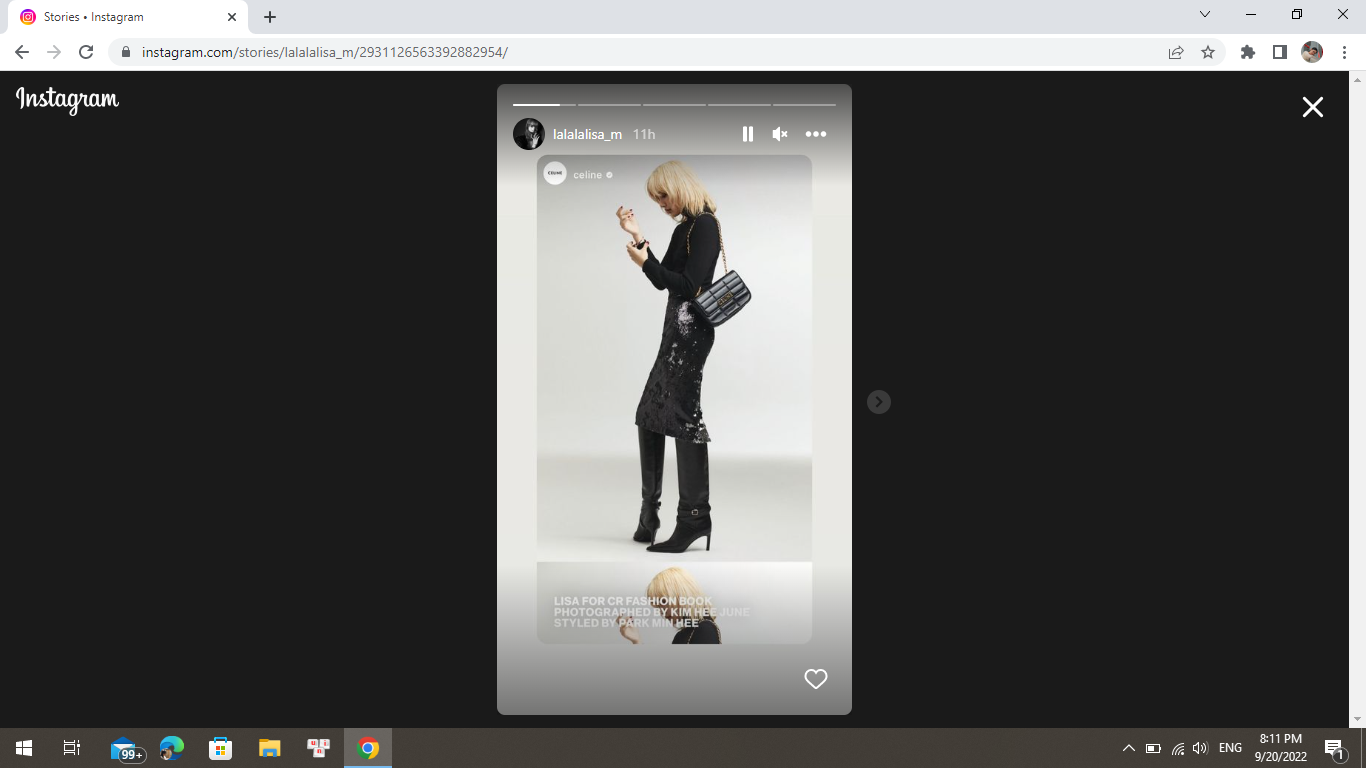
\includegraphics[width=13cm]{Images/chapter 2/instagram/story_web.png}
        \caption{Story trên web}
        \label{fig:my_label}
    \end{figure}
\\
\newpage
    \item \textbf{Tích hợp công cụ nhắn tin.} Bạn có thể nhắn tin, trò chuyện cùng bạn bè người thân, với những người mình yêu quý và có chung sở thích qua Instagram. Ngoài ra, bạn có thể sử dụng tính năng gọi video call để trò chuyện miễn phí ngay trên ứng dụng.
\end{itemize}

\subsubsection{Ưu điểm và nhược điểm}
\subsubsubsection{Ưu điểm}
\textbf{Những điểm nổi bật của Instagram so với facebook:}
\begin{itemize}
    \item Chỉ với một bức ảnh bạn bè có thể đoán được tâm trạng của bạn đang vui hay buồn.
    \item Nếu như Facebook chủ yếu là chia sẻ cảm xúc của bạn bằng những status thì Instagram chỉ cần một bức ảnh mọi người đã biết bạn đang cảm thấy như thế nào. Đây chính là một yếu tố khiến Instagram thu hút hơn Facebook.
    \item Hiện tại Instagram đã cập nhật tính năng cho phép bạn ghi lại hình ảnh của bạn trong vòng 15 giây. Bạn có thể ghi lại một video khoảng 15 giây và nói một điều gì đó thú vị. Hiện tại Instagram chưa phát triển hết khả năng video nhưng trong những thời gian tới có lẽ chức năng quay video sẽ có thời gian dài hơn 15 giây.
    \item Instagram sử dụng rất đơn giản, người lớn tuổi cũng có thể dễ dàng sử dụng. Bạn chỉ cần bấm vào Instagram, chạm vào biểu tượng máy ảnh, chụp một tấm và nhấn tải ảnh lên.
    \item Instagram được ưa thích hơn facebook là nhờ 19 hiệu ứng chỉnh sửa ảnh. Bạn có thể tìm thấy một hiệu ứng hoàn hảo cho bất kỳ bức ảnh nào của mình. Những hiệu ứng này chắc chắn sẽ làm bạn cảm thấy hào hứng và hài lòng.
    \item Instagram có ứng dụng Emoji giúp bạn thêm một khuôn mặt cười hay ngón tay hướng lên trên để thể hiện cảm xúc khi bức ảnh của bạn bè bạn đăng lên mà không biết phải bình luận như thế nào.
    \item Instagram cũng cho phép bạn bè của bạn biết rằng: Bạn đang tồn tại, bạn đang làm gì? Bạn đang đi đâu?
    \item Với Instagram, bạn có thể nhìn thế giới qua đôi mắt của người khác, điều đó thực sự rất tuyệt vời.
    \item Khi dùng Instagram bạn không phải bắt gặp những tin spam liên quan đến quảng cáo. Tại đây, bạn sẽ được thỏa sức định hình phong cách cá nhân của mình. Ngay cả khi phong cách đó là những bức ảnh không sử dụng hiệu ứng hay chỉnh sửa.
\end{itemize}
\\ \par
\newline
\textbf{Với những phân tích và khảo sát, có thể đúc kết được Instagram có các ưu điểm như sau:}
\begin{itemize}
    \item Là một mạng xã hội lớn, phổ biến rộng rãi, được lượng lớn người dùng ưu chuộng.
    \item Hình ảnh có khả năng gợi lên cảm xúc, hấp dẫn hơn các hình thức tương tác khác
    \item Công cụ tiếp thị tốt, nhiều cửa hàng ảo sử dụng nền tảng này để quảng bá sản phẩm của họ.
    \item Chú trọng về quyền riêng tư và bảo mật. Đây là một trong những lợi thế quan trọng của Instagram.
    \item Ứng dụng hoàn toàn miễn phí cho người dùng.
    \item Phương tiện giao tiếp tốt với các tính năng gọi, call video, phát livestream.
\end{itemize}
\subsubsubsection{Nhược điểm}
\textbf{Bên cạnh những ưu điểm đã phân tích, còn tồn tại một số nhược điểm:}
\begin{itemize}
    \item Instagram được thiết kế dành cho ứng dụng là chủ yếu, đối với phiên bản trên web thì Instagram không cung cấp nhiều dịch vụ như ứng dụng di động.
    \item Không tương thích với tất cả các hệ điều hành. Instagram chỉ khả dụng trên IOS, Android và Windows Mobile, điều này không bao gồm những người có thiết bị có hệ thống BlackBerry, OS và Linux.
    \item Khả năng trộm cắp hình ảnh. Khi đăng tải những  bức ảnh đẹp, chất lượng và chuyên nghiệp lên mạng xã hội, đặc biệt là mạng xã hội phát triển như Instagram thì việc bị đánh cắp hình ảnh mà không có sự đồng ý của chính chủ là rất phổ biến. 
    \item So với các mạng xã hội như Facebook, zalo thì Instagram không cung cấp tính năng group chat. Bạn chỉ có thể chat trực tiếp với 1 người.
    \item Instagram chứa nhiều trang cửa hàng ảo, dẫn tới việc quảng cáo nhiều, có khi thông tin sai lệch.
    \item Giống với các mạng xã hội khác thì Instagram còn có tiềm năng gây nghiện cho người dùng, dẫn tới phụ thuộc vào mạng xã hội.
\end{itemize}

\par 

\subsection{Pinterest}
Pinterest là một xã hội được thiết kế để quản lý và chia sẻ ý tưởng về hình ảnh, ra mắt vào năm 2009. 
Hình ảnh được chia sẻ thông qua thao tác được gọi là pin (ghim).\par \par 


\textbf{Điểm nổi bật của Pinterest:}
\begin{itemize}
    \item Home Feed có thuật toán tìm ảnh tương đương.
    \item Thuật toán gợi ý chủ đề theo theo từ khóa tìm kiếm.
    \item Tính năng “Pin”: “Pin” về cơ bản có nghĩa là bạn lưu trữ một bộ sưu tập hình ảnh với nhau để tạo thành một nhóm. Mỗi hình ảnh riêng lẻ là một pin mà người khác đã đưa lên. Tính năng Pin áp dụng cho tất cả ảnh xuất hiện ở Home Feed hoặc mục tìm kiếm.
    \item Tính năng follow tác giả.
    \item Bảng: tính năng lưu trữ và chia sẻ tập hợp tất cả các Pin. các Pin công khai được hiển thị trên trang Profile.
\end{itemize}

\subsubsection{Ưu điểm và nhược điểm}
    \subsubsubsection{Ưu điểm}
        \begin{itemize}
            \item Pinterest rất dễ sử dụng, quá trình đăng nhập cũng không mất nhiều thời gian.
            \item Đây là kênh mạng xã hội có khả năng lưu giữ một lượng lớn hình ảnh cho người dùng.
            \item Pinterest hữu ích để quảng bá sản phẩm và kinh doanh online.
            \item Theo thống kế, Pinterest có tới hơn 81\% người dùng là nữ giới nên là môi trường tiềm năng để tiếp thị các sản phẩm làm đẹp.
        \end{itemize}

    \subsubsubsection{Nhược điểm}
        \begin{itemize}
            \item Vì là mạng xã hội chủ yếu lưu giữ hình ảnh nên Pinterest hoàn toàn là các hình ảnh theo chủ đề người dùng yêu thích.
            \item Hình ảnh của người dùng không được bảo vệ bản quyền vì không có công cụ hỗ trợ.
        \end{itemize}



\par 

\subsection{Behance}


Behance được thành lập vào năm 2006 bởi Adobe. Đây được xem là một mạng xã hội dành cho các nhà thiết kế,
 những người yêu thích cái đẹp và sự sáng tạo. Bạn có thể tạo một tài khoản của riêng mình và đăng tải những
  hình ảnh mà bạn đã thiết kế, đây có thể được xem như là một Portfolio chuyên nghiệp dành cho dân thiết kế.






\subsubsection{Ưu điểm và nhược điểm}
\subsubsubsection{Ưu điểm}
\subsubsubsection{Nhược điểm}

\par 

\subsection{YouPic}
YouPic được thành lập vào năm 2012 bởi Giám đốc điều hành hiện tại là Navi Razazi. 
Công ty có trụ sở chính tại Gothenburg, là thành phố lớn thứ hai ở Thụy Điển. 
YouPic có hơn ba triệu người dùng trên khắp thế giới.\par

Về bản chất, nền tảng này hoạt động giống như sự giao thoa giữa Twitter và Instagram. 
Ngoài tính chất chia sẻ hình ảnh, người dùng có thể chia sẻ lại và like những bức hình mình yêu thích.\par

Nền tảng này được thiết kế để giúp các nhiếp ảnh gia không chỉ chia sẻ tác phẩm của họ mà còn nhận được phản hồi. 
YouPic cũng cho phép người dùng được thuê cho công việc của khách hàng, trong khi quyền hình ảnh vẫn thuộc 
về nhiếp ảnh gia sau khi xuất bản.\par

Youpic không chỉ là một nền tảng truyền thông xã hội dành cho các nhiếp ảnh gia mà nó còn có rất nhiều 
khía cạnh truyền thông xã hội đa dạng khác. Giống như các đối tác của Youpic, bạn có thể sử dụng nó để trình
 bày hình ảnh mà mọi người có thể chia sẻ và tương tác.\par

Điều khiến Youpic trở nên khác biệt với các trang web thông thường là nó phục vụ chủ yếu cho các chuyên
 gia hơn là nhiếp ảnh gia nghiệp dư. Nó đóng vai trò như một đường dẫn trong việc trao đổi ý tưởng với các 
 nhiếp ảnh gia và thậm chí cả những khách hàng trong tương lai.\par

Trang mạng xã hội này chứa đầy những thứ mà ngay cả bản thân các bức ảnh cũng bao gồm thông tin kỹ thuật như 
dữ liệu EXIF và thẻ địa lý.\par

Ngoài việc chia sẻ ảnh, nó cho phép bạn truy cập vào các hướng dẫn từ những người giỏi nhất trong lĩnh vực kinh 
doanh. Ngoài ra, bạn cũng có thể kiếm tiền từ ứng dụng bằng cách bán công việc hoặc dịch vụ của mình.\par


\subsubsection{Ưu điểm và nhược điểm}
\subsubsubsection{Ưu điểm}
\subsubsubsection{Nhược điểm}

    \newpage

    % \section{Tổng quan}

\subsection{Lý do lựa chọn đề tài}
Mạng xã hội đã trờ thành một phần không thể thiếu trong cuộc sống của chúng ta ngày nay. 
Nó là một công cụ giao tiếp có giá trị với những người khác trong nước và trên toàn thế giới, cũng như để chia sẻ,
 tạo và truyền bá thông tin.\par 
Hiện nay, với sự phát triển mạnh mẽ của các thiết bị điện tử và ngành du lịch, khách tham quan từ nhiều nơi khác nhau 
sẽ đến những điểm du lịch để có những trải nghiệm mới, việc chụp ảnh để lưu giữ lại kỉ niệm cùng với người thân, bạn bè 
từ đó cũng là điều không thể thiếu. Vậy chúng ta lưu giữ và chia sẻ hình ảnh ở đâu?\par 
Instagram hiện nay được cho là nền tảng mạng xã hội phổ biến nhất để lưu giữ, xem những hình ảnh, video từ bạn bè và 
những nhân vật công chúng mà chúng ta thấy hấp dẫn và thú vị. Bên cạnh đó, Pinterest là website rất phổ biến để lưu giữ, 
chia sẻ ảnh theo dạng mạng xã hội, dùng để post và phân loại dưới dạng các đính kèm.
Cả hai mạng xã hội đều đang có một nhược điểm khác nhau. Instagram thì không tập trung toàn bộ vào chia sẻ hình ảnh, 
các chức năng mạng xã hội chỉ dừng ở việc chia sẻ, nhắn tin. Trong khi đó thì Pinterest tập trung vào mảng hình ảnh nhưng lại 
thiếu các chức năng của mạng xã hội.\par
Do đó, chúng tôi muốn xây dựng một mạng xã hội dành cho cộng đồng những người yêu thích chụp ảnh. Tại đây, mọi người 
có thể chia sẻ những bức ảnh đẹp do chính họ chụp được, những công thức riêng cho một bức ảnh đẹp, những kiến thức về máy ảnh 
và cách chụp ảnh. Ngoài ra, người dùng có thể tìm kiếm,  bình luận, chia sẻ, nhắn tin,  lập các hội nhóm chung sở thích để chi sẻ, 
học hỏi kinh nghiệm. Mạng xã hội này sẽ khắc phục nhửng nhược điểm của hai mạng xã hội trên, kết hợp những ưu điểm để tạo ra một nơi 
mà những người yêu thích chụp ảnh chắc chắn sẽ tìm tới.


\subsection{Lý do lựa chọn đề tài}
Từ những nội dung trên, một số vấn đề được đề cập và giải quyết trong đề tài này:
    \begin{itemize}
        \item Làm thế nào bảo vệ bản quyền cho ảnh của người dùng và cho nền tảng?
        \item Làm cách nào để xây dựng giải thuật tìm kiếm dựa vào ảnh tương tự?
        \item Làm sao để ứng dụng đáp ứng được mục tiêu: là nơi để cộng đồng đam mê nhiếp ảnh có thể chia sẻ ảnh và kinh nghiệm chụp ảnh?
        \item Những tính năng nào của mạng xã hội đòi hỏi có trong ứng dụng?
    \end{itemize}

Để thực hiện được mục tiêu này, chúng tôi đã đề ra những nhiệm vụ cần phải giải quyết như sau:
    \begin{itemize}
        \item Nghiên cứu và ứng dụng auto watermarking, hoặc hạn chế người dùng chụp màn hình.
        \item Xây dựng nền tảng cung cấp đầy đủ các tính năng mạng xã hội và ưu tiên phát huy tối đa tính năng lưu giữ và chia sẻ hình ảnh.
        \item Xây dựng hệ thống ổn định và đáng tin cậy
    \end{itemize}


\subsection{Lý do lựa chọn đề tài}
Phạm vi nghiên cứu của đề tài nhóm sẽ tìm hiểu về lĩnh vực mạng xã hội, các nội dung về lĩnh vực nhiếp ảnh.\par
Đối tượng nghiên cứu chủ yếu của đề tài sẽ dành cho tất cả mọi người có yêu thích về nhiếp ảnh và 
có cơ hội muốn tìm hiểu về nhiếp ảnh, Instagram và Pinterest
    

    % \newpage

    


%\thispagestyle{empty}

% \newpage
% wdwdwe
% \newpage

% \tableofcontents


% \newpage


% \section{GIỚI THIỆU DỰ ÁN THƯƠNG MẠI ĐIỆN TỬ}
% \subsection{Tổng quan dự án trong bối cảnh Thương mại điện tử trong nước hiện nay}
% Trước tình hình COVID-19 hiện tại, vấn đề học tập trực tuyến đang diễn ra khá phổ biến. Ở trường Đại học Bách Khoa, chương trình học cũng khá nặng, mỗi buổi học thì các bạn sinh viên cần phải tiếp thu rất nhiều kiến thức. Do đó, một số bạn có khả năng tiếp thu chậm hơn thì sẽ dễ bị ngộp và dẫn đến chán nản. Do đó ConceptCourse sinh ra nhằm giúp các bạn củng cố kiến thức, giúp các bạn có hứng thú hơn khi học môn học đó.

% \subsubsection{Ý nghĩa và động lực của dự án}
% Nền tảng học tập trực tuyến là một không gian web hoặc cổng thông tin cho nội dung và tài nguyên giáo dục cung cấp cho sinh viên mọi thứ họ cần ở một nơi: bài giảng, tài nguyên, cơ hội gặp gỡ và trò chuyện với các sinh viên khác, v.v. Đây cũng là một cách tuyệt vời để học sinh và giáo viên theo dõi sự tiến bộ của học sinh.

% Học trực tuyến mang lại nhiều lợi ích:
% \begin{itemize}
% 	\item Giá rẻ
% 	\item Sự thoải mái khi làm việc tại nhà
% 	\item Tự học theo nhịp độ
% 	\item Cải thiện kỹ năng kỹ thuật, giao tiếp và tư duy phản biện
% 	\item Kỹ năng quản lý thời gian tốt hơn và hơn thế nữa
% \end{itemize}


% Nền tảng giáo dục cập nhật phải có tích hợp với:
% \begin{itemize}
% 	\item Lịch trực tuyến (Google, Calendly) để có cơ hội lên lịch cuộc gọi và trò chuyện, thiết lập lời nhắc và chọn ngày hoàn thành công việc, v.v.
% 	\item Lưu trữ đám mây (Google, Dropbox)
% 	\item Mạng xã hội (LinkedIn, Facebook) để kích hoạt chức năng chia sẻ xã hội và hoàn thiện hồ sơ người dùng
% \end{itemize}
% \subsubsubsection {Quản lý theo thời gian thực}
% Trang tổng quan thống kê là một bảng trực tiếp để hiển thị số liệu thống kê của người dùng thông qua biểu đồ và sơ đồ. Trang tổng quan được sử dụng để theo dõi hoạt động của chuyên gia, xếp hạng, tỷ lệ thành công của người học, các môn học phổ biến nhất, v.v. Trang này cũng được nhóm hỗ trợ nền tảng sử dụng cho các nhu cầu nội bộ.

% \subsubsection{Thuận lợi, khó khăn}
% \subsubsubsection{Thuận lợi}
% Đã từng có nhiều trải nghiệm với những nền tảng học trực tuyến
% \subsubsubsection{Khó khăn}
% Tìm kiếm nguồn tài liệu, giảng viên đáng tin cậy
% \newpage
% \subsection{Khảo sát người dùng về động lực và ý tưởng của dự án}
% \begin{figure}[!htp]
% 	\centering
% 	\includegraphics[width=15cm]{research-1.png}
% \end{figure}




% \section{BUSINESS MODEL CANVAS}
% \subsection{Customer Segments}
% \begin{itemize}
% 	\item Sinh viên, học sinh muốn bổ sung kiến thức
% 	\item Sinh viên, học sinh không có thời gian đến làm muốn tự học tại nhà
% \end{itemize}
% \subsection{Value Propositions}
% \begin{itemize}
% 	\item Học và giảng dạy trực tuyến
% 	\item Học ở mọi nơi, mọi lúc
% 	\item Các khóa học là các môn học đại cương được giảng dạy tại các chương trình đại học
% 	\item Mỗi khóa học được tổ chức theo từng chủ đề với bài tập chủ đề tương ứng
% \end{itemize}
% \subsection{Channels}
% \begin{itemize}
% 	\item Internet
% 	\item Facebook: các trang đoàn hội của khoa, trường
% 	\item Website
% 	\item Email
% \end{itemize}
% \subsection{Customer Relationships}

% \begin{figure}[!htp]
% 	\centering
% 	\includegraphics[width=15cm]{canvas.png}
% \end{figure}



% \section{XÂY DỰNG KẾ HOẠCH TIẾP THỊ SỐ - BÁN HÀNG}
% \subsection{Các hoạt động cần thực hiện}
% \subsubsection{Liên hệ với các đối tác tạo sản phẩm khóa học}
% Liên hệ các giáo viên, giảng viên đại học, giáo sư, phó giáo sư, thạc sĩ, tiến sĩ có kinh nghiệm trong môn học cụ thể để hợp tác với công ty tạo ra sản phẩm là khóa học online theo tiêu chí của doanh nghiệp.\\
% Ưu tiên lựa chọn các đối tác chuyên môn về khóa học nhằm mục đích tối ưu hóa chất lượng của sản phẩm
% \subsubsection{Liên hệ với các đội tác marketing}
% Chạy quảng cáo Affiliate, SEO trên các nền tảng web giáo dục như : Udemy, Geeksforgeeks, hoặc các trang web riêng của các trường học, đại học, cao đẳng, nghề.\\
% Quảng bá sản phẩm trên các nền tảng thương mại điện thiên về giáo dục.
% \subsection{Đối tác liên kết}
% \subsubsection{Đối tác liên kết tạo ra sản phẩm}
% Giáo viên, giảng viên đến từ các trường trung học phổ thông, đại học, cao đẳng, trường nghề.\\
% Các chuyên gia về từng lĩnh vực cụ thể, ví dụ : tạo ra một khóa học mạng máy tính cần ít nhất 1 chuyên gia về mạng máy tính và ít nhất 1 giảng viên đại học đã từng dạy bộ môn mạng máy tính và có kinh nghiệm dạy học.\\
% Các bạn sinh viên năm cuối chuyên ngành cụ thể, ví dụ : tạo ra một khóa học Toeic 450 cần tối thiểu 1 bạn sinh viên năm cuối chuyên ngành ngôn ngữ Anh hoặc các bạn sinh viên chuyên ngành sư phạm Anh, hoặc các bạn sinh viên có yêu thích ngôn ngữ và có TOEIC 700+ và có kinh nghiệm giảng dạy ít nhất 1 năm.\\



% \section{CHI PHÍ ƯỚC TÍNH}
% \subsection{Chi phí mua tên miền}
% Tên miền là dòng chữ mà người dùng nhập vào các trình duyệt trên Internet để truy cập đến website của bạn. Mỗi website đều cần có địa chỉ website riêng, địa chỉ này cũng giống như địa chỉ nhà, rõ ràng dễ nhớ và đặc biệt nó không trùng lặp với các địa chỉ website khác. Website sẽ có tên miền Việt Nam (.vn). Do đó, chi phí thuê tên miền rơi vào khoảng 600.000 VNĐ.


% \section{TRIỂN KHAI THỬ NGHIỆM}
% \textbf{Tích hợp Google Analytic vào trang web}
% \subsection{Cách tích hợp}
% \noindent Bước 1: Tạo tài khoản \textbf{Google Analytic}: Vào trang  \href{https://analytics.google.com/}{https://analytics.google.com/} và bấm \textbf{Bắt đầu đo lường}
% \begin{figure}[!htp]
% 	\centering
% 	\includegraphics[width=14cm]{GA1.png}
% 	\caption{}
% 	\label{fig:my_label}
% \end{figure}

% \newpage
% \noindent Bước 2: Bạn điền \textbf{tên tài khoản} tùy ý rồi nhấp \textbf{Tiếp theo}.\\
% \begin{figure}[!htp]
% 	\centering
% 	\includegraphics[width=14cm]{GA2.png}
% 	\caption{}
% 	\label{fig:my_label}
% \end{figure}

% \newpage
% \noindent Bước 3: Bạn điền \textbf{Tên thuộc tính} tùy ý rồi chọn múi giờ là Việt Nam (GMT+07), chọn đơn vị tiền tệ là VND sau đó bấm \textbf{Tiếp theo}.\\
% \begin{figure}[!htp]
% 	\centering
% 	\includegraphics[width=14cm]{GA3.png}
% 	\caption{}
% 	\label{fig:my_label}
% \end{figure}
% \newpage
% \noindent Bước 4: Chọn quy mô doanh nghiệp và loại ngành. Ở đây chúng ta sẽ chọn quy mô từ 1 - 10 nhân viên. Sau đó bấm \textbf{Tạo}\\
% \begin{figure}[!htp]
% 	\centering
% 	\includegraphics[width=14cm]{GA4.png}
% 	\caption{}
% 	\label{fig:my_label}
% \end{figure}


% \section{PHỤ LỤC}
% \subsection{Tài liệu tham khảo}
% \subsection{Link giao diện}
% \href{https://conceptcourse.netlify.app/}{conceptcourse.netlify.app/}
% \subsection{Link source code}
% \href{https://github.com/bao-nguyenbku/e-commerce.git}{github.com/bao-nguyenbku/e-commerce.git}
% \subsection{Video demo sản phẩm}
% \href{}{}
% \subsection{Bảng phân công nhiệm vụ và đánh giá}
% \begin{center}
% 	\begin{tabular}{ |c|c|m{13em}|c| }
% 		\hline
% 		\textbf{STT} & \textbf{Họ và tên}  & \textbf{Công việc}                                                                                                                   & Đánh giá \\
% 		\hline
% 		1            & Nguyễn Thiên Bảo   & Xây dựng kiến trúc thông tin, code giao diện MVP                                                                               & 100\%       \\
% 		\hline
% 		2            & Quang Chấn Vĩ        & Xây dựng business canvas model, code tích hợp Paypal, SMS email                                                                   & 100\%       \\
% 		\hline
% 		3            & Trịnh Duy Hưng       & Hoàn thiện động lực và ý tưởng của dự án, code giao diện học online                                               & 100\%       \\
% 		\hline
% 		4            & Lê Trung Hiếu        & Lập kế hoạch các hoạt động cần thực hiện, đối tác liên kế, thời gian                                         & 100\%       \\
% 		\hline
% 		5            & Nguyễn Ngô Gia Bảo & Chi phí ước tính: từ chuẩn bị, khởi tạo, thiết kế, xây dựng, triển khai, vận hành, tiếp thị, quảng bá & 100\%       \\
% 		\hline
% 		6            & Nguyễn Thái Linh     & Thiết kế kiến trúc thông tin                                                                                                    & 100\%       \\
% 		\hline
% 		7            & Vũ Huy Hoàng          & Xây dựng business canvas model                                                                                                       & 100\%       \\
% 		\hline
% 	\end{tabular}
% \end{center}
\end{document} 